%%%%%%%%%%%%
%%%%%%%%%%%%
\begin{figure}
\centering
%%%%%%%%%%%%
\pgfdeclarelayer{background}
\pgfsetlayers{background,main}
%%%%%%%%%%%%
%%%%%%%%%%%%

\begin{subfigure}[t]{.3\textwidth}
	\centering
	\fbox{\includegraphics[width=\textwidth]{fig/lorenz/t5.png}}
    	\caption{$t=5$}
	\label{fig:rayleigh_field_0}
\end{subfigure} \quad
\begin{subfigure}[t]{.3\textwidth}
	\centering
	\fbox{\includegraphics[width=\textwidth]{fig/lorenz/t25.png}}
    	\caption{$t=25$}
	\label{fig:rayleigh_field_2}
\end{subfigure} \quad
\begin{subfigure}[t]{.3\textwidth}
	\centering
	\fbox{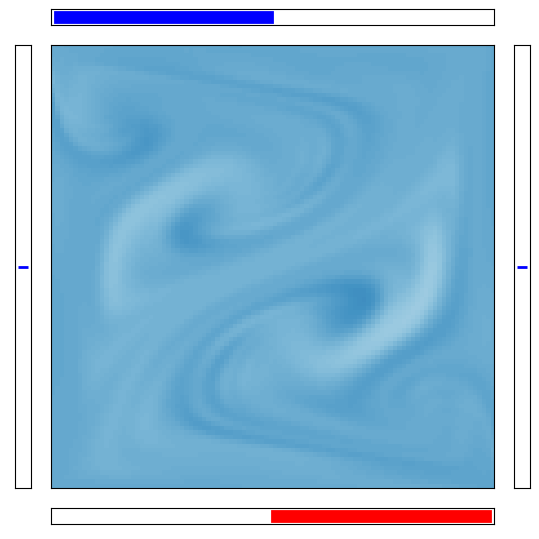
\includegraphics[width=\textwidth]{fig/lorenz/t50.png}}
    	\caption{$t=50$}
	\label{fig:rayleigh_field_4}
\end{subfigure}

\medskip

\begin{subfigure}[t]{.3\textwidth}
	\centering
	\fbox{\includegraphics[width=\textwidth]{fig/lorenz/t100.png}}
    	\caption{$t=100$}
	\label{fig:rayleigh_field_8}
\end{subfigure} \quad
\begin{subfigure}[t]{.3\textwidth}
	\centering
	\fbox{\includegraphics[width=\textwidth]{fig/lorenz/t200.png}}
    	\caption{$t=200$}
	\label{fig:rayleigh_field_10}
\end{subfigure} \quad
\begin{subfigure}[t]{.3\textwidth}
	\centering
	\fbox{\includegraphics[width=\textwidth]{fig/lorenz/t300.png}}
    	\caption{$t=300$}
	\label{fig:rayleigh_field_12}
\end{subfigure}

%%%%%%%%%%%%
\caption{\textbf{Evolution of the controlled Lorenz system} using the \ppo algorithm. The instantaneous control value is indicated at the bottom by the colored bar (blue is for $-1$, red is for $+1$).}
\label{fig:lorenz_fields}
\end{figure} 
%%%%%%%%%%%%
%%%%%%%%%%%%